\documentclass[12pt,twoside]{article}
\usepackage{jmlda}
\newcommand{\hdir}{.}
\usepackage{hyperref}       % clickable links
\usepackage{lineno}
\usepackage{graphicx,multicol}
\usepackage{cite}

\usepackage{tikz}
\usetikzlibrary{shapes,arrows,shadows}

\bibliographystyle{jmlda_eng}
%\renewcommand{\baselinestretch}{1.4}

\newcommand{\bz}{\mathbf{z}}
\newcommand{\bx}{\mathbf{x}}
\newcommand{\by}{\mathbf{y}}
\newcommand{\bw}{\mathbf{w}}
\newcommand{\bY}{\mathbf{Y}}
\newcommand{\bX}{\mathbf{X}}
\newcommand{\ba}{\mathbf{a}}
\newcommand{\bu}{\mathbf{u}}
\newcommand{\bt}{\mathbf{t}}
\newcommand{\bp}{\mathbf{p}}
\newcommand{\bq}{\mathbf{q}}
\newcommand{\br}{\mathbf{r}}
\newcommand{\bg}{\mathbf{g}}
\newcommand{\bh}{\mathbf{h}}
\newcommand{\bb}{\mathbf{b}}
\newcommand{\bv}{\mathbf{v}}
\newcommand{\be}{\mathbf{e}}
\newcommand{\bc}{\mathbf{c}}
\newcommand{\bP}{\mathbf{P}}
\newcommand{\bT}{\mathbf{T}}
\newcommand{\bQ}{\mathbf{Q}}
\newcommand{\bE}{\mathbf{E}}
\newcommand{\bF}{\mathbf{F}}
\newcommand{\bU}{\mathbf{U}}
\newcommand{\bI}{\mathbf{I}}
\newcommand{\bB}{\mathbf{B}}
\newcommand{\bW}{\mathbf{W}}
\newcommand{\bD}{\mathbf{D}}
\newcommand{\bH}{\mathbf{H}}
\newcommand{\bG}{\mathbf{G}}
\newcommand{\bZ}{\mathbf{Z}}
\newcommand{\bJ}{\mathbf{J}}
\newcommand{\bM}{\mathbf{M}}
\newcommand{\btheta}{\boldsymbol{\theta}}
\newcommand{\bmu}{\boldsymbol{\mu}}
\newcommand{\blambda}{\boldsymbol{\lambda}}
\newcommand{\bPsi}{\boldsymbol{\Psi}}
\newcommand{\bpsi}{\boldsymbol{\psi}}
\newcommand{\bsigma}{\boldsymbol{\sigma}}
\newcommand{\bSigma}{\boldsymbol{\Sigma}}
\newcommand{\bphi}{\boldsymbol{\phi}}
\newcommand{\bdelta}{\boldsymbol{\delta}}


\title
	{Снижение размерности пространства зависимой переменной в задачах прогнозирования.}
\author
	{Мария Владимирова}
\email
    {\href{mailto:mrvladimirova@gmail.com}{mrvladimirova@gmail.com}}
\organization
    {Московский физико-технический институт}
\abstract
	{Решается задача обнаружения способов зависимостей в прогнозируемой переменной. Используется набор гомогенных моделей, восстанавливающих прогноз по общему для всех переменных описанию объектов. Анализируется различие в пространстве параметров моделей. По результатам анализа выбирается оптимальная структура каждой модели. 

    \bigskip
	\noindent
	\textbf{Ключевые слова}: \emph {multitask learning, partial least squares, многозадачность, ... } 
	}

\thanks{Проект поддержан грантом РФФИ \No 16-07-01155.}


%\bibliographystyle{unsrt}

\begin{document}
\maketitle




% \title
% 	{Bagging of Neural Networks for Analysis of Nuclear Receptor Biological Acivity}
% \author
% 	{Maria Vladimirova, Maria Popova}
% \email
%     {\href{mailto:mrvladimirova@gmail.com}{mrvladimirova@gmail.com},  \href{mailto:popova@gmail.com}{popova@gmail.com}}
% \organization
%     {Moscow Institute of Physics and Technology}
% \abstract
% 	{The paper is devoted to the multitask classification problem. 
% 	The main purpose is building an adequate model to predict whether the object belongs to a particular class. 
% 	Precisely, whether the ligand binds to a specific nuclear receptor. 
% 	Nuclear receptors are a class of proteins found within cells. 
% 	These receptors work with other proteins to regulate the expression of specific genes, thereby controlling the development, homeostasis, and metabolism of the organism. 
% 	The regulation of gene expression generally only happens when a ligand~---~a molecule that effects the receptor’s behavior~---~binds to a nuclear receptor.
% 	Two layer neural network is used as a classification model. 
% 	The paper considers the problems of linear and logistic regressions with squared and cross-entropy loss functions. 
% 	To analyze the classification result we propose to decompose the error into bias and variance terms. 
% 	To improve the quality of classification by reducing the error variance we suggest the composition of neural networks: the bagging procedure.  
% 	The proposed method improves the quality of investigated sample classification.

%     \bigskip
% 	\noindent
% 	\textbf{Key words}: \emph {nuclear receptors, biological activity, two layer neural network, bagging, multi-task learning, drug-design, cross-entropy} 
% 	}

% \thanks{This research is funded by RFBR, grant 16-07-01155.}



%\linenumbers

\section{1. Introduction}

	Electric energy is a significant driving force for economic development, while the accuracy of demand forecasts is an important factor leading to the success of efficiency planning. For this reason, energy analysts need a guideline to better choose the most appropriate forecasting techniques in order to provide accurate forecasts of electricity consumption trends. 
	
	Concept named multitask learning (MTL)~\cite{Adolph, Evgeniou2007} (\textit{refer to an article, e.g. Caruana, R. Multitask learning.}
	% Mach. Learn. 1997, 28 (1), 41− 75.
	) was proposed to use the redundancy information.

	MTL can be carried out using machine learning methods yielding models with several independent outputs, such as neural networks, another type of inductive transfer, uses extra tasks to build the models, predictions of which are further used as extra inputs for the main task~\cite{Varnek2012}. (\textit{refer to chemometrics})

	There is the multitask learning method of giving extra information through the model’s outputs in artificial neural networks, where extra outputs are trained in parallel with the main task outputs while using a shared representation~\cite{Caruana2003}(\textit{Caruana, 2003}). Many learning methods do not have representation naturally shared between tasks. \cite{Adolph} (\textit{Learning to learn}) presents an algorithm and results for MTL with case-based methods such as $k$-nearest neighbor and kernel regression, and sketches an algorithm for MTL in decision tree induction.  


	In this letter, we focus on the multitask problem using Partial Least Squares (PLS) regression method.
	The goal of PLS regression \cite{Abdi2003}(\textit{Abdi}) is to predict $\bY$ from $\bX$ and to describe their common structure. When $\bY$ is a vector and $\bX$ is a full rank matrix, this goal could be accomplished using ordinary multiple regression. When the number of predictors is large compared to the number of observations, $\bX$ is likely to be singular and the regression approach is no longer feasible because of multicollinearity. 

	For the history of PLS and about PLS regression see~\cite{Geladi1988, Hoskuldsson1988}(\textit{Geladi}) and (\textit{Höskuldsson}). 
	The difference between PLS and related technique, different varieties of PLS regression can be viewed in~\cite{Lehky2014}(\textit{Bayesian PLS}).
	MTL using PLS regression method was proposed to address the multivariate calibration problems in the analytical chemistry in~\cite{Lu2004}(\textit{MTL using PLS}). 

	A nonlinear extension of the PLSR method is firstly introduced in~\cite{Frank1990}. A lot of PLS methods were developed in the literature. The activation functions of artificial neural networks are used in PLS method. Because the activation functions provide highly nonlinear transformations, they solve multicollinearity problem. Moreover, PLS method has non-linear modeling ability. Paper proposes non-linear PLS method based on defferent methods: feed forward artificial neural networks ~\cite{Mcavovt1992}, radial bases activation functions\cite{Yan2003}, logistic activation function and particle swarm optimization methods~\cite{Zhou2007}, differently use feed forward neural networks~\cite{Xuefeng2010}, Elman feedback artificial neural networks~\cite{Bulut2014}.

\section{2. Problem statement}

\subsection{2.1 Partial Least Squares Regression}
	Partial Least Squares (PLS) regression finds components from $\bX$ that are also relevant for $\bY$. Specifically, PLS regression searches for a set of components (called latent vectors) that performs a simultaneous decomposition of $\bX$ and $\bY$ with the constraint that these components explain as much as possible of the covariance between $\bX$ and $\bY$. This step generalizes PCA. It is followed by a regression step where the decomposition of $\bX$ is used to predict $\bY$.	

	The general underlying model of multivariate PLS is
	\[
		\bX = \bT \bP^{\T} + \bE,
	\]
	\[
		\bY = \bU \bQ^{\T} + \bF,
	\]
	where $\bX$ is an $n\times m$ rank matrix of predictors, $\bY$ is an $n\times p$ matrix of responses. $\bT$ and $\bU$ are $n\times l$ score matrices that are, respectively, projections of $\bX$ and projections of $\bY$, $\bT^{\T} \bT = \bI$. $\bP$ and $\bQ$ are, respectively, $m \times l$ and $p \times l$ orthogonal loading matrices. $\bB$ is diagonal matrix with ``regression weights'' as diagonal elements and matrices $\bE$ and $\bF$ are the error terms, assumed to be independent and identically distributed random normal variables. 
	The columns of $\bT$ are called latent vectors. When their number is equal to the rank  of $\bX$, they perform an exact decomposition of $\bX$. The decompositions of $\bX$ and $\bY$ are made so as to maximise the covariance between $\bT$ and $\bU$. Specifically, the goal is to obtain a first pair of vectors $\bt = \bX \bp$ and $\bu = \bY \bq$ with the constraints that $\bp^{\T}\bp = 1$, $\bt^{\T}\bt = 1$ and $\bt^{\T}\bu$ be maximal.

	Iterative process:
	\begin{multicols}{2}
		% $\bt_0 = \bx_1$

		% while $t_k$ changes:

		% $\bp_k = \bX^{\T} \bt_{k-1} / \| \bX^{\T} \bt_{k-1} \|$

		% $\bt_k = \bX \bp_k$

		% $\bu_0 = \by_1$

		% while $u_k$ changes:

		% $\bq_k = \bY^{\T} \bu_{k-1}/ \| \bY^{\T} \bu_{k-1} \|$

		% $\bu_k = \bY \bq_k$

	\begin{enumerate}
		\item $\bw = \bX^{\T} \bu / (\bu^{\T} \bu)$
		\item $\| \bw \| \to 1$
		\item $\bt = \bX \bw$
		\item $\bc = \bY^{\T} \bt / (\bt^{\T} \bt)$
		\item $\| \bc \| \to 1$
		\item $\bu = \bY \bc$
	\end{enumerate}
	\end{multicols}

	By $\mathbf{T} = \mathbf{U} \bB$, $\bP \sim \bX^{\T} \mathbf{U}$ and $\mathbf{Q} \sim \bY^{\T} \mathbf{T}$. To preserve relation $\mathbf{T} = \mathbf{U} \bB$ between $\mathbf{T}$ and $\mathbf{U}$  one may use the following fused procedure: set $\bu_0 = y_1,\ k = 1$ and while $\bt_k$ changes, repeate:
	% \begin{multicols}{0}

		% $\bp_k = \bX^{\T} \bu_{k-1} / \| \bX^{\T} \bu_{k-1} \|$

		% $\bt_k = \bX \bp_k$

		% $\bq_k = \bY^{\T} \bt_k / \|\bY^{\T} \bt_k\|$

		% $\bu_k = \bY \bq_k,\ k = k + 1$
	% \end{multicols}
	\begin{equation*}
		\bp = \bX^{\T} \bt / (\bt^{\T} \bt), \quad \bq = \bY^{\T} \bu / (\bu^{\T} \bu)
	\end{equation*}

	Then we have 
	\begin{equation*}
		\bp = \bX^{\T}\bu = \bX^{\T} \bY \bq = \bX^{\T} \bY \bY^{\T} \bt = \bX^{\T} \bY \bY^{\T} \bX \bp / \|\bX^{\T} \bY \bY^{\T} \bX\|,
	\end{equation*}
	which is update rule for the eigenvector of the covariance matrix of $\bY^{\T} \bX$. In [\textit{Kee Siong Ng}] shown that $\bp$ is is the solution to the optimisation problem 
	\begin{equation}
	\label{opt_pls}
		\argmax\limits_{\| \bp \| = 1} \bp^{\T}\bX^{\T}\bY\bY{\T}\bX \bp =
		\argmax\limits_{\| \bp \| = 1}  \text{Var} (\bX \bp)(\text{Corr} (\bY, \bX \bp))^{\T} \text{Corr} (\bY, \bX \bp) 
	\end{equation}
	
	The most frequently used variant of linear PLS is based on two assumptions i) the score vectors ${\bt_i}_{i=1}^p$ are good predictors of $\bY$, and ii) a linear inner relation between the scores vectors $\bt$ and $\bu$ exists; that is,
	\begin{equation}
	\label{inner_relation_lin}
		\bU = \bT \bD + \bH
	\end{equation}
	where $\bD$ is the $p \times p$ diagonal matrix and $\bH$ denotes the matrix of residuals.


\tikzstyle{sensor_x}=[draw, fill=blue!0, text width=7em, 
    text centered, minimum height=8.5em,drop shadow]
\tikzstyle{sensor_y}=[draw, fill=blue!0, text width=5em, 
    text centered, minimum height=8.5em,drop shadow]

\def\blockdist{2.3}
\def\edgedist{2.5}

\begin{tikzpicture}
    \node (x) [sensor_x]  {$\bX$};
    \path (x.south)+(0,-3) node (tilde_x) [sensor_x] {$\tilde \bX$};
    \path (x.east)+(5,0) node (y) [sensor_y] {$\bY$};
    \path (y.south)+(0,-3) node (tilde_y) [sensor_y] {$\tilde \bY$};
    \path (tilde_x.south)+(0,-1.1) node (x_form) {$\bX = \bT \bP^{\T} + \bE$};
    \path (tilde_y.south)+(0,-1.1) node (y_form) {$\bY = \bU \bQ^{\T} + \bM$};
    \path (tilde_x.south)+(3.5,-2) node (u_form) {$\bU = \bT \bD + \bZ$};


    \path [draw, ->] (x.south) -- node [right] {$f_x(\bX, \bv_x)$} 
        (tilde_x.north);
    \path [draw, ->] (y.south) -- node [right] {$f_y(\bY, \bv_y)$} 
        (tilde_y.north);
    %tilde X
    \path [draw, -] +(1.8,-3) -- node [right] {$\bt$}
    	+(1.8,-6.5);
    \path [draw, -] +(1.6,-6.7) -- node [below] {$\bp$}
    	+(-1.6,-6.7); 
   	%tilde Y
    \path [draw, -] +(5.25,-3) -- node [left] {$\bu$}
    	+(5.25,-6.5);
    \path [draw, -] +(5.4,-6.7) -- node [below] {$\bq$}
    	+(7.8,-6.7);

    \path [draw, ->] +(1.6,-6.5) -- node [above] {$\bw$}
    	+(3.3,-8.3);
    \path [draw, ->] +(5.4,-6.5) -- node [above] {$\bc$}
    	+(2.5,-8.3);
\end{tikzpicture}

\section{3 Pre-training}
	Let us consider monotone functions \ref{table_functions}.
% \begin{table}[]
% \centering
% \label{table_functions}
% \begin{tabular}{|l|l|l|l|l|}
% \hline
% \textbf{Форма отклика} & \textbf{Функция}                    & \textbf{Параметры} & $x'$       & $y'$     \\ \hline
% Очень быстрый рост     & $f = \exp(a + bx)$                  & $b > 0$            & $x$        & $\ln f$  \\ \hline
% Быстрый рост           & $f = \exp(a + b \ln x)$             & $b > 1$            & $\ln x$    & $\ln f$  \\ \hline
% Медленный рост         & $f = \exp(a + b \ln x)$             & $0 < b < 1$        & $\ln x$    & $\ln f$  \\ \hline
% Очень медленный рост   & $f = a + bx$                        & $b > 0$            & $\ln x$    & $f$      \\ \hline
% Медленная стабилизация & $f = a + b / x$                     & $b \not= 0$        & $1 / x$    & $f$      \\ \hline
% Быстрая стабилизация   & $f = a + b \exp(-x)$                & $b \not= 0$        & $\exp(-x)$ & $f$      \\ \hline
% Сигмоида               & $f = 1 / \bigl(a + b\exp(-x)\bigr)$ & $b > 0$            & $\exp(-x)$ & $ 1 / f$ \\ \hline
% \end{tabular}
% \caption{Монотонные модели}
% \end{table}

\begin{table}[h]
\label{table_functions}
\centering
\begin{tabular}{|l|l|l|l|l|}
\hline
\textbf{Response form} & \textbf{Function}                   & \textbf{Parameters} & $x'$       & $y'$     \\ \hline
Very fast growth       & $g = \exp(a + bx)$                  & $b > 0$             & $x$        & $\ln g$  \\ \hline
Fast growth            & $g = \exp(a + b \ln x)$             & $b > 1$             & $\ln x$    & $\ln g$  \\ \hline
Slow growth            & $g = \exp(a + b \ln x)$             & $0 < b < 1$         & $\ln x$    & $\ln g$  \\ \hline
Very slow growth       & $g = a + b \ln x$                   & $b > 0$             & $\ln x$    & $g$      \\ \hline
Slow stabilization     & $g = a + b / x$                     & $b \not= 0$         & $1 / x$    & $g$      \\ \hline
Fast stabilization     & $g = a + b \exp(-x)$                & $b \not= 0$         & $\exp(-x)$ & $g$      \\ \hline
Sigmoid                & $g = 1 / (a + b\exp(-x))$ & $b > 0$             & $\exp(-x)$ & $ 1 / g$ \\ \hline
\end{tabular}
\caption{Monotone functions}
\end{table}

\subsection{3.0 The dependent variable transformation}

	
\[\begin{diagram}
\node{\bY}
\arrow{e,t}{g_y(\bY, \bv_y)}
\node{\breve \bY}
\arrow{e,t}{h_y(\breve \bY)}
\node{\tilde \bY}
\end{diagram}\]

	% \begin{equation*}
	% 	\bY \under{\longrightarrow}^ \breve \bY \tilde \bY
	% \end{equation*}

	Firstly, consider curvelinear transformation with vector of parameters $\bv_y$
	\begin{equation}
	\label{transf_y}
		\breve \bY = g_y (\bY, \bv_y) = \bG_y(\bY, \bv_y),
	\end{equation}
	then, nonparametric transformation 
	\begin{equation*}
		\tilde \bY = h_y (\breve \bY) = h_y (g_y (\bY, \bv_y)) = f_y(\bY, \bv_y)
	\end{equation*}

	The second-order Taylor expansion of (\ref{transf_y}) has the form
	\begin{equation*}
		\breve \by = \breve \by_{0} + \frac{\partial g_y}{\partial \bv_y} \Big|_{0} \Delta \bv_y,
	\end{equation*}
	where $\breve \by_{0} = g_y(\bt)$ is the value of $g_y$ at the known value of $\by$.
	The following steps to compute $\Delta \bv$ were suggested. The approach considers the difference $\breve \by - \breve \by_{0} = \frac {\partial g_y}{\partial \bv_y} \Big|_{0} \Delta \bv$ at the first step. Next, this leads to the following definition of a mismatch $\be$
	\begin{equation*}
		\be = \breve \by - \breve \by_{0} = \frac {\partial g_y}{\partial \bv_y} \Big|_{0} \Delta \bv_y = \bJ_{y} \Delta \bv_y,
	\end{equation*}
	where $\bJ_{y}$ consists of the partial derivatives $\left\{\frac {\partial g}{\partial v_i}\Big|_{0} \right\}_{i=1}^N$. From this mismatch relation $\Delta \bv_y$ can be directly computed by regressing the mismatch $\be$ on $\bJ_{y}$ 
	\begin{equation}
	\label{delta_v}
		\Delta \bv_y  = (\bJ^{\T}_{y} \bJ_{y})^{-1} \bJ_{y}^{\T} \be.
	\end{equation}


\subsection{3.1 Stacked Nonlinear Autoencoders}
	A stacked autoencoder is a neural network consisting of multiple layers of sparse autoencoders in which the outputs of each layer is wired to the inputs of the successive layer. 

	Let $W_{ij}^{(l)}$ denote the parameter (or weight) associated with the connection between unit $j$ in layer $l$, and unit $i$ in layer $l+1$. Also, $b_i^{(l)}$ is the bias associated with unit $i$ in layer $l+1$, $a_i^{(l)}$ is the activation of unit $i$ in layer $l$. For $l = 1$, we also use $a_i^{(1)} = x_i$ to denote the $i$-th input. 


	Define autoencoder $\bg(\bx)$ as a superposition
	\begin{align*}
		\ba^{(2)} = f(\bW^{(1)} \bx + \bb^{(1)}) - \text{encoder}, \\
		\bg(\bx)  = f(\bW^{(2)} \ba^{(2)} + \bb^{(2)}) - \text{decoder},
	\end{align*}
	where $\bW^{(1)}, \bW^{(2)}$, $\bb^{(1)}, \bb^{(2)}$ are autoencoder parameter. We consider nonlinear autoencoders where $f$ is a function from table \ref{table_functions}.


	Also let $\bz^{(l)}$ denote the total weighted sum of inputs to unit $i$ in layer $l$, including the bias term (e.g., $\bz^{(2)} =  \bW^{(1)} \bx + \bb^{(1)}$), so that $\ba^{(l)} = f(\bz^{(l)})$.


	% \begin{equation*}
	% 	\bmu = \bphi (\bg (\bx)),
	% \end{equation*}
	% where 
	% \begin{equation*}
	% 	\mathbf{g}(\mathbf{x}) = \boldsymbol{\sigma}(\mathbf{W}_g\mathbf{x}+\mathbf{b}_g) - \text{encoder},
	% \end{equation*}
	% \begin{equation*}
	% \label{decoder}
	% \boldsymbol{\varphi}(\mathbf{g}(\mathbf{x})) = \boldsymbol{\sigma}(\mathbf{W}_h\mathbf{g}(\mathbf{x})+\mathbf{b}_h) - \text{decoder},
	% \end{equation*}
	% $\mathbf{W}_g$, $\mathbf{W}_{\varphi}$, $\mathbf{b}_g$, $\mathbf{b}_{\varphi}$ are autoencoder parameters, $\boldsymbol{\sigma}(\mathbf{t}) = \dfrac{1}{1 + \exp(-\mathbf{t})}$ is sigmoid fuction.

	To optimize the autocoder parameters $\mathbf{\Theta} = (\mathbf{W}^{(1)}, \mathbf{W}^{(2)}, \mathbf{b}^{(1)}, \mathbf{b}^{(2)})$, we need to select the initial approximation for the parameters of each block separately, and then adjust the parameters of the whole model as a whole by the backpropagation method.

	The autoencoder tries to learn a function $\bg_{\mathbf{\Theta}}(\bx) \approx \bx$. In other words, it is trying to learn an approximation to the identity function, so as to output $\hat{\bx}$ that is similar to $\bx$ 
	\begin{equation*}
		\|\mathbf{g}(\bx |\mathbf{\Theta}) - \mathbf{x}\|^2_2 \to \min\limits_{\mathbf{\Theta}}.
	\end{equation*}
	
	Let $\mathbf{\Theta}^{(k)} = (\mathbf{W}^{(k,1)}, \mathbf{W}^{(k,2)}, \mathbf{b}^{(k,1)}, \mathbf{b}^{(k,2)})$ denote the parameters $\mathbf{W}^{(1)}, \mathbf{W}^{(2)}, \mathbf{b}^{(1)}, \mathbf{b}^{(2)}$ for $k$-th autoencoder.  Then the encoding step for the stacked autoencoder is given by running the encoding step of each layer in forward order:
	\begin{align*}
	\mathbf{a}^{(l)} = f(\bz^{(l)}), \\
	\bz^{(l + 1)} = \mathbf{W}^{(l, 1)}\mathbf{a}^{(l)} + \mathbf{b}^{(l, 1)}.
	\end{align*}
	The decoding step is given by running the decoding stack of each autoencoder in reverse order:
	\begin{align*}
	\mathbf{a}^{(n + l)} = f(\bz^{(n + l)}), \\
	\bz^{(n + l + 1)} = \mathbf{W}^{(n - l, 2)}\mathbf{a}^{(n + l)} + \mathbf{b}^{(n - l, 2)}.
	\end{align*}

	Thus, the stacked autoencoder result is
	\[
		\mathbf{f}_{\mathbf{\Theta}} (\bx) = \ba_{\mathbf{\Theta}^{(n)}} (\dots \ba_{\mathbf{\Theta}^{(1)}}(\bx)\dots),
	\]
	where $\mathbf{\Theta} = (\mathbf{\Theta}^{(1)}, \dots, \mathbf{\Theta}^{(n)})$ are stacked autoencoder parameters. The result of $k$-th encoder is $\bx^{(k)} = \ba_{\mathbf{\Theta}^{(k)}}(\bx^{(k - 1)}), \bx^{(1)} = \bx$.

	The purpose is to minimize the following system
	% \begin{equation*}
	% S(\mathbf{\Theta}, \mathbf{x}) = \sum\limits_{k=1}^n\|\mathbf{g}(\bx^{(k)} |\mathbf{\Theta}^{(k)}) - \mathbf{x}\|^2_2.
	% \end{equation*}
	\begin{equation*}
		S(\mathbf{\Theta}^{(k)}, \mathbf{x}^{(k)}) = \|\mathbf{g}(\bx^{(k)} |\mathbf{\Theta}^{(k)}) - \ba^{(k)}\|^2_2 \to \min\limits_{\mathbf{\Theta}}, \ \ k \in \{1, \dots, n\}.
	\end{equation*}
	Thus,
	\begin{equation*}
	\hat{\mathbf{\Theta}}^{(k)} =  \mathop{\text{argmin}}\limits_{\mathbf{\Theta}} \dfrac{1}{2|\mathcal{L}|} \sum_{\mathbf{x} \in \mathcal{L}} S(\mathbf{\Theta}^{(k)}, \mathbf{x}^{(k)}), \ \ k \in \{1, \dots, n\}.
	\end{equation*}




\subsection{3.2 Nonlinear PLS (nlPLS)}
	
	Extend the linear PLS model to its nonlinear form by replacing the linear inner relation (\ref{inner_relation_lin}) between the score vectors $\bt$ and $\bu$ by a nonlinear model 
	\begin{equation}
	\label{inner_pls_nl}
		\bu = g_x(\bt) + \bz = g_x(\bX, \bv_x) + \bz,
	\end{equation}
	where $g_x$ represents a continuous nonlinear function, $\bz$ denotes a vector of residuals and $\bw$ is a vector of weights. The fuction $g_x(\bX)$ is a parametric matrix $\bG_x(\bX) = \bG_x(\bX, \bv_x)$ where $\bv_x$ is a solution of optimization PLS problem~(\ref{opt_pls}). 

	The second-order Taylor expansion of (\ref{inner_pls_nl}) has the form
	\begin{equation*}
		\bu = \bu_{0} + \frac{\partial g_x}{\partial \bv_x} \Big|_{0} \Delta \bv_x,
	\end{equation*}
	where $\bu_{0} = g_x(\bt)$ is the value of $g_x$ at the known value of $\bt$.
	The following steps to compute $\Delta \bv$ were suggested. The approach considers the difference $\bu - \bu_{0} = \frac {\partial g_x}{\partial \bv} \Big|_{0} \Delta \bv$ at the first step. Next, this leads to the following definition of a mismatch $\be$
	\begin{equation*}
		\be = \bu - \bu_{0} = \frac {\partial g_x}{\partial \bv_x} \Big|_{0} \Delta \bv_x = \bJ_{x} \Delta \bv_x,
	\end{equation*}
	where $\bJ_{x}$ consists of the partial derivatives $\left\{\frac {\partial g}{\partial v_i}\Big|_{0} \right\}_{i=1}^N$. From this mismatch relation $\Delta \bv_x$ can be directly computed by regressing the mismatch $\be$ on $\bJ_v$ 
	\begin{equation}
	\label{delta_v}
		\Delta \bv_x  = (\bJ^{\T}_x \bJ_v)^{-1} \bJ_x^{\T} \be.
	\end{equation}


\subsection{3.3 Curvelinear PLS (clPLS)}
	Extend the linear PLS model to its nonlinear form by replacing the linear inner relation~(\ref{inner_relation_lin}) between the score vectors $\bt$ and $\bu$ by a nonlinear model 
	\begin{equation}
	\label{inner_pls_nonlin}
		\bu = g_x(\bt) \bw  + \bh = g_x(\bX) \bw + \bh.
	\end{equation}
	The function $g_x(\bX) = \bG_x$ is a nonparametric matrix and $\bw$ is a vector of weights.

	The following step to compute $\Delta \bw$ was suggested:
	\begin{equation}
	\label{delta_w}
		\Delta \bw = (\bG_x^{\T} \bG_x)^{-1} \bG_x^{\T} \bu.
	\end{equation}


\subsection{3.4 nclPLS}
	Extend the nonlinear PLS model to its curvelinear form by replacing the linear inner relation~(\ref{inner_pls_nl}) between the score vectors $g(\bt)$ and $\bu$ by a nonlinear model 
	\begin{equation}
	\label{inner_pls_ncl}
		\bu = g_x(\bt) \bw  + \bz = g_x(\bX, \bv_x) \bw + \bz.
	\end{equation}
	
	The previous steps in nlPLS~(\ref{delta_v}) and clPLS~(\ref{delta_w}) are proposed to be used in the nclPLS method.
	Finnaly, the whole nclPLS method starts from random initialization of $\bu$ and the following steps are repeated until convergence

	\begin{multicols}{2}
	\begin{enumerate}
		\item $\bw = \bX^{\T} \bu / (\bu^{\T} \bu )$

		\item $\| \bw \| \to 1$

		\item $\bt = \bX \bw$

		\item fit $g_x(\cdot)$ using $\bu, \bt$

		\item $\bu_{0} = g_x(\bt)$

		\item $\bc = \bY^{\T} \bu_{0} / (\bu_{0}^{\T} \bu_{0})$

		\item $\| \bc \| \to 1$

		\item $\be = \bu - \bu_{0}$ 

		\item compute $\bJ_x$

		\item $\Delta \bv_x = (\bJ_x^{\T} \bJ_x)^{-1} \bJ_x^{\T} \be$

		\item $\bu = \bu_{0} + \bJ_x \Delta \bv$

		\item $\Delta \bw = (\bG_x^{\T} \bG_x)^{-1} \bG_x^{\T} \bu$

		\item $\bw = \bw + \Delta \bw$

		\item go to step 2.
	\end{enumerate}
	\end{multicols}
 

% \subsection{3.2 Self-organizing map (SOM)}
% 	The Self-Organizing Map (SOM), commonly also known as Kohonen network (Kohonen 1982, Kohonen 2001) is a computational method for the visualization and analysis of high-dimensional data, especially experimentally acquired information.
% 	% It is a type of artificial neural network that is trained using unsupervised learning to produce a low-dimensional, discretized representation of the input space of the training samples, called a map, and is therefore a method to do dimensionality reduction. Self-organizing maps differ from other artificial neural networks as they apply competitive learning as opposed to error-correction learning (such as backpropagation with gradient descent), and in the sense that they use a neighborhood function to preserve the topological properties of the input space.

% 	The SOM uses a set of neurons, often arranged in a 2D rectangular or hexagonal grid, to form a discrete topological mapping of an input space, $\bX \in \mathbb{R}^n$. At the start of the learning, all the weights $\{\bw_{r1}, \bw_{r2}, \dots, \bw_{rm}\}$ are initialised to small random numbers. $\bw_{ri}$ is the weight vector associated to neuron $i$ and is a vector of the same dimension, $n$, of the input. $m$ is the total number of neurons. $\br i$ is the location vector of neuron $i$ on the grid. Then the algorithm repeats the following steps.
	
% 	\begin{itemize}
% 	\item At each time $t$, present an input, $\bx(t)$, select the winner, 
% 	\begin{equation*}
% 		v(t) = \argmin_{k \in \Omega} \|\bx(t) - \bw_k (t)\|.
% 	\end{equation*}
% 	\item Updating the weights of winner and its neighbours,
% 	\begin{equation*}
% 		\Delta \bw_k (t) = \alpha(t) \eta(v, k, t)[\bx(t) - \bw_v (t)].
% 	\end{equation*}
% 	\item Repeat until the map converges,
% 	\end{itemize}
% 	where $\eta(v, k, t)$ is the neighbourhood function, $\Omega$ is the set of neuron indexes and $\alpha(t)$ is a learning restraint due to iteration progress.

\section{4. Experiment}
	В рамках вычислительного эксперимента строится прогноз временных рядов. В ходе эксперимента сравниваются методы PLSR, нелинейных автоэнкодеров и нелинейной коррекции. Сравнение проводится на реальных данных объемов потребления электроэнергии в Польше и на реальных данных ECoG сигналов. 

\subsection{4.1 ``Energy-Weather'' Dataset }
	The computational experiments demonstrated in this section are based on the Energy-Weather data set (Available: http://gdudek.el.pcz.pl/varia/stlf-data). The dataset consists of the Polish electricity load time series and weather time series in Warsaw (Longtitude: 21.25, Latitude: 52.30, Elevation: 94). Energy time series contain hourly records (total of 52512 observations), while weather time series were measured daily and contain 2188 observations. The multiscale time series correspond to the period of 1999 to 2004. The results observed on this data set are illustrative of the proposed framework since the data set contains the time series that are both multiscale and have various nature.

	Here are results of the baseline method: for time series the next forecasted value is predicted with the most recent observed value.
	

	\begin{figure}[!h]
		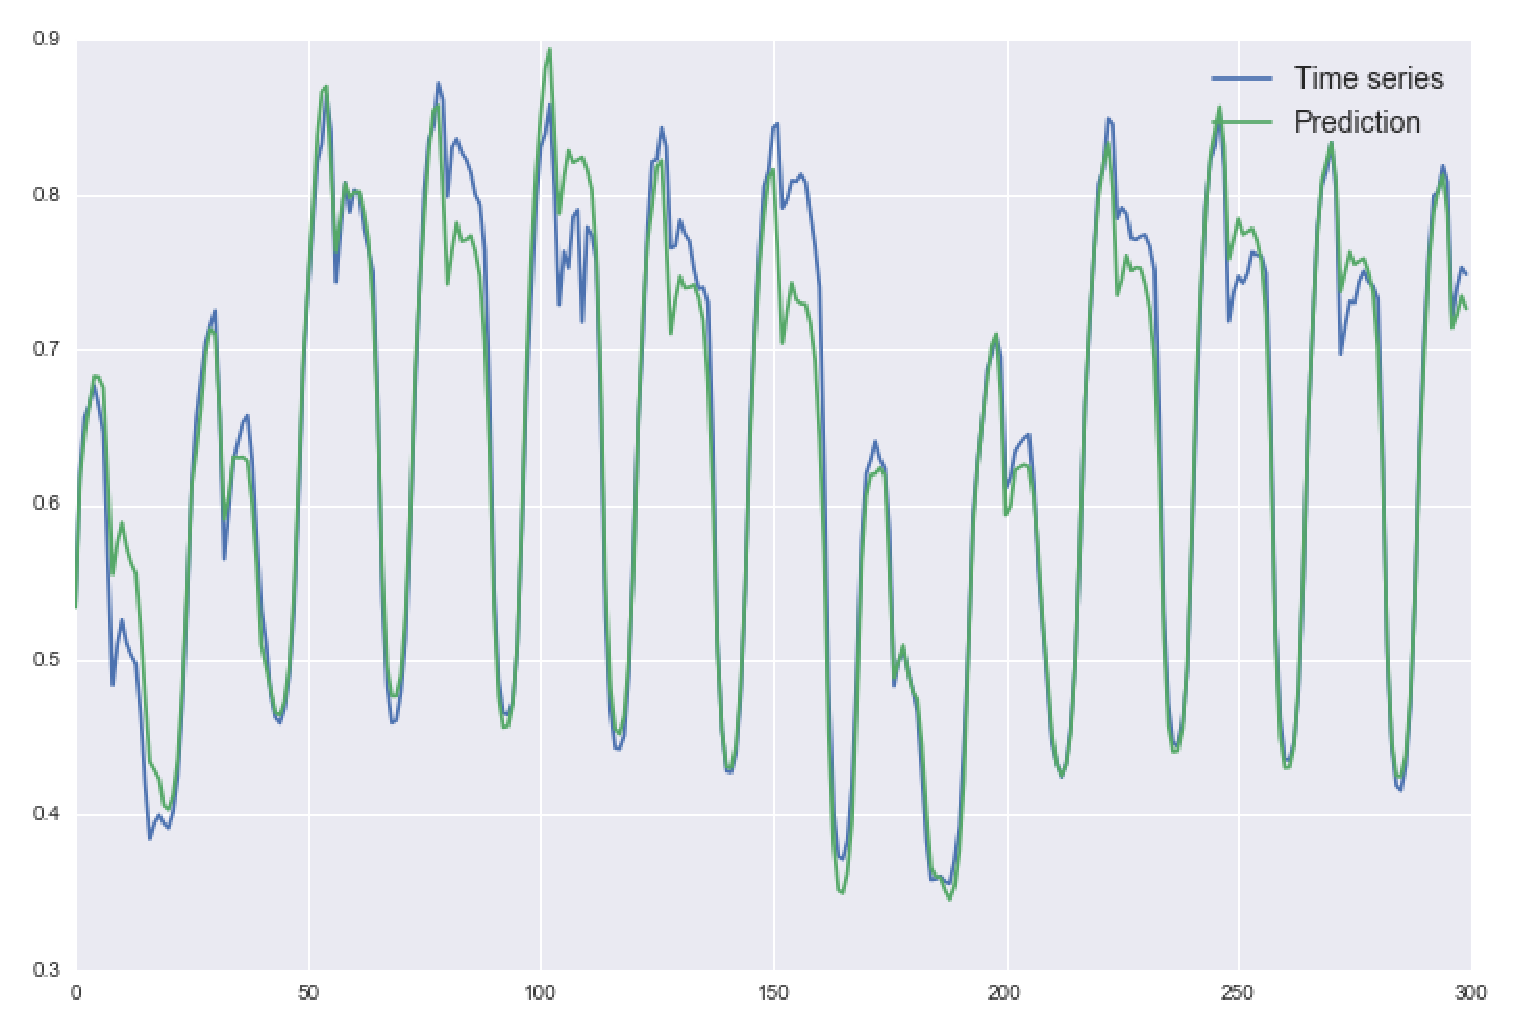
\includegraphics[width=0.9\textwidth]{prediction_pls.eps}
	\caption{PLS Regression, ``Energy-Weather'' Dataset }
	\end{figure}

\subsection{4.2 ``ECoG'' Dataset }

	The monkey was tracking food rewards with the hand contralateral to the implant side. ECoG data and motion data were recorded simultaneously during the task ({\textit reference}) (Available: http://neurotycho.org/social-competition-task). There was no eye tracking. ECoG and motion data were sampled at 1KHz and 120Hz, respectively, with time stamps synchronized. 

	Data format: 
	\begin{itemize}
	\item ECoG\_chN.mat

	ECoGData\_chN: ECoG signal ($\mu V$) recorded from electrode $N$ (1‐64), sampled at 1kHZ.
	The Location of electrode is documented in ``B.png''.

	\item ECoG\_time.mat

	ECoGTime: ECoGTime is a one row-vector contains Time-stamps with the same length as ECoGData\_chN.

	\item Motion.mat

	MotionData: MotionData is a time $\times$ marker matrix containing $3D$ position of marker (index 1, LSHO: left shoulder, index 2, LELB: left elbow, index 3, LWRI: left wrist, index 4, RSHO: right shoulder, index 5, RELB: right elbow, index 6, RWRI: right wrist).

	MotionTime: MotionTime contains the corresponding time-stamps.

	\begin{figure}[!h]
	\center
		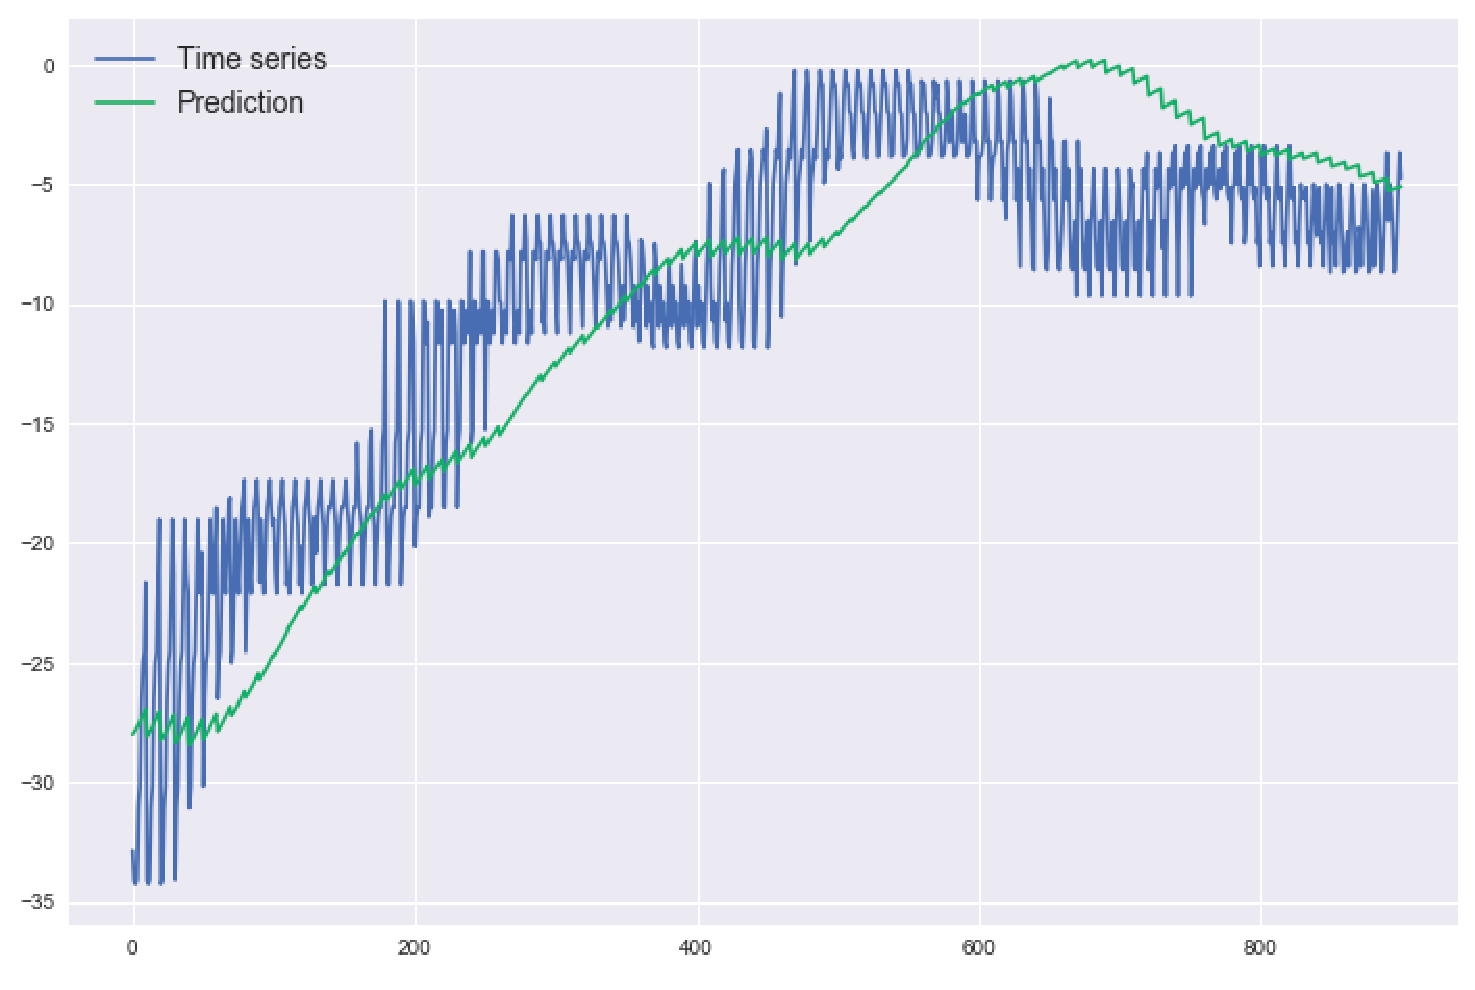
\includegraphics[width=0.9\textwidth]{prediction_pls_ecog.eps}
	\caption{PLS Regression, ``ECoG'' Dataset, 1 electrode}
	\end{figure}


	\end{itemize}
\newpage
\nocite{*}
\renewcommand{\bibname}{References}
\bibliography{papers}



% \newpage
% \maketitle

% \nocite{*}
% \renewcommand{\bibname}{References}
% \bibliography{papers}


\end{document}